Here the protocol presented by Giordani et al. \cite{giordani2020} is summarised.
The aim of the protocol is to generate higher dimensional entanglement via the use of quantum walks.
The imagined setup of this protocol is that there are two labs, $A$ and $B$, which have a shared source of entangled qubits but are otherwise spatially separated and cannot interact with one another.

In this section the following notation is employed:
\begin{itemize}
    \item $\ket{\psi}_J$ is a state belonging to the subspace $\mathcal{H}_J = \mathcal{H}^{(A)}_J \otimes \mathcal{H}^{(B)}_J, J\in\{C,W\}$. It is a state that describes the combined state of the coins or walkers.
    \item $\ket{\psi}^{(K)}$ is a state belonging to the subspace $\mathcal{H}^{(K)} = \mathcal{H}^{(K)}_C \otimes \mathcal{H}^{(K)}_W, K\in\{A,B\}$. It is a state that describes the combined state of one of the quantum walks.
    \item  $\ket{\psi}^{(K)}_J$ is a state belonging to the subspace $\mathcal{H}^{(K)}_J$.
\end{itemize}

In this mathematical framework the overall Hilbert space is comprised of two quantum walk subspaces,
\begin{align}
    \mathcal{H} &= \mathcal{H}^{(A)} \otimes \mathcal{H}^{(B)}\\
                &= \mathcal{H}^{(A)}_C \otimes \mathcal{H}^{(A)}_W \otimes \mathcal{H}^{(B)}_C \otimes \mathcal{H}^{(B)}_W.
\end{align}
Due to the difficulty, however, in writing entangled states when the entangled spaces are not adjacent, states will be written with the following ordering
\begin{equation}
    \mathcal{H} = \mathcal{H}^{(A)}_W \otimes \mathcal{H}^{(B)}_W \otimes \mathcal{H}^{(A)}_C \otimes \mathcal{H}^{(B)}_C,
\end{equation} 
i.e. with the walker subspaces adjacent to each other and the coin subspaces adjacent to each other.

The basic premise of this protocol is this:
\begin{enumerate}
    \item Entangle the two coin spaces of the walkers $\mathcal{H}^{(K)}_C$. (Figure \ref{fig:preparation}.)
    \item Proceed with the quantum walk for some determined number of steps.
    \item Use a projective measurement $\mathcal{P}_\gamma = \ket{\gamma}\bra{\gamma}, \ket{\gamma}\in\mathcal{H}^{(A)}_C$ to then transfer the entanglement so that it solely exists in the subspace $\mathcal{H}^{(A)}_W \otimes \mathcal{H}^{(B)}_C \otimes \mathcal{H}^{(B)}_W$.
    \item In similar fashion, find a projection $\mathcal{P}_\delta = \ket{\delta}\bra{\delta}, \ket{\delta}\in\mathcal{H}^{(B)}_C$ to transfer the entanglement to exist between the two walker subspaces, $\mathcal{H}^{(i)}_W$, only.
    \item Accumulate entanglement in the walker subspaces by once more entangling the two coin spaces and repeating the protocol.
\end{enumerate}

\begin{figure}
    \centering
    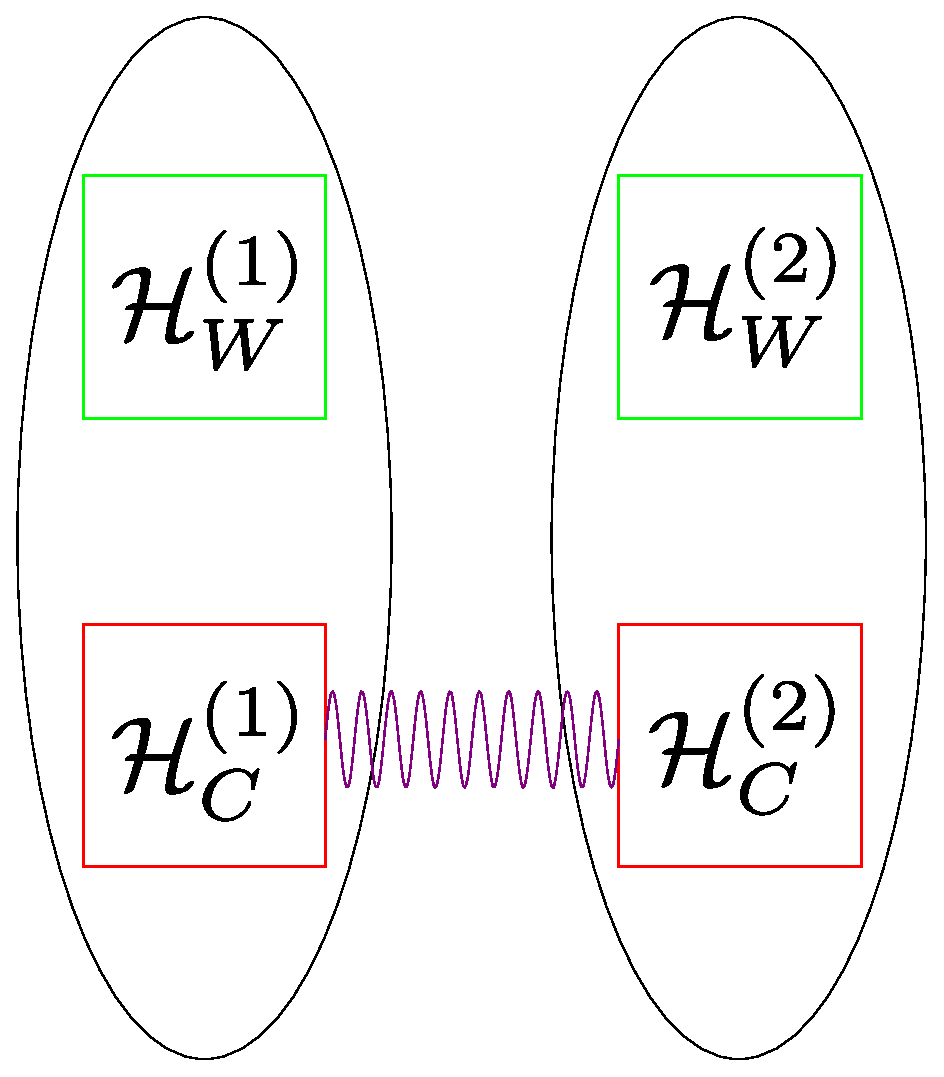
\includegraphics[scale = .25]{preparation}
    \caption{The initial prepared state has entanglement solely between the two coin subspaces. Figure is an edited version of FIG 3 from \cite{giordani2020}.}
    \label{fig:preparation}
\end{figure}
In this way, arbitrary amounts of higher dimensional entanglement can be generated.\newline
The ordering of steps 3 and 4 is not overly important since the full operators describing the projective measurements are given by
\begin{align}
    &\ket{\gamma}\bra{\gamma} \otimes I \otimes I \otimes I,\\
    &I \otimes \ket{\delta}\bra{\delta} \otimes I \otimes I
\end{align}
which clearly commute.
As is the case with many quantum walk based protocols, particular attention must be paid to the choice of coin used for the quantum walk, as it will have a large impact on the success of the protocol.
The shift operator used for the quantum walks is $\tilde{S}$, as outlined in section \ref{subsubsection:q_r_w}.
(Technically it is $\tilde{S}\otimes\tilde{S}$, one for each walk, but for the sake of brevity $\tilde{S}$ will be used.)

\subsection{Transfer using identity coin operator}
\label{subsection:qw_transfer}
To illustrate the basic principles of the protocol, consider the case where 
\begin{equation}
    C = \underbrace{I_2 \otimes I_2}_{\text{"Coin" operators}} \otimes I_d \otimes I_d = I.
\end{equation}
Note that this is not actually an instance of using quantum walk dynamics, since an identity coin equates to no coin at all.

\begin{enumerate}
    \item A state $\ket{\psi(0)}$ is prepared with the walkers at the origin and coin states entangled,
    \begin{equation}
        \ket{\psi(0)} = \ket{0}^{(A)}_W\ket{0}^{(B)}_W \otimes \underbrace{\frac{1}{\sqrt{2}}\Big [\ket{\uparrow}^{(A)}_C\ket{\uparrow}^{(B)}_C + \ket{\downarrow}^{(A)}_C\ket{\downarrow}^{(B)}_C \Big]}_{\text{Bell State}}.
    \end{equation}
    \item The "coin", $I$, is applied and followed by the shift operator $\tilde{S}$ to advance the quantum walk.
    Explicitly (dropping the indices and combining kets together) the walk evolves to the state
    \begin{equation}
        \ket{\psi(1)} = \tilde{S}I\ket{\psi} = \frac{1}{\sqrt{2}}\Big [\ket{0,0}\ket{\uparrow,\uparrow} + \ket{1,1}\ket{\downarrow,\downarrow}\Big].
    \end{equation}
    \item Using the operator $\mathcal{P}_{\gamma} = \ket{\gamma}\bra{\gamma}$ the part of $\ket{\psi(1)}$ residing in the $\mathcal{H}^{(A)}_C$ subspace is projected onto the state $\ket{\gamma}$.
    
    For this example, choose $\ket{\gamma} = \frac{1}{\sqrt{2}} \big [\ket{\uparrow} + \ket{\downarrow} \big]$ which then gives
    \begin{equation}
        \mathcal{P}_\gamma \ket{\psi(1)} = \frac{1}{2}\Big [\ket{0, 0}\ket{\gamma,\uparrow} + \ket{1, 1}\ket{\gamma, \downarrow}\Big ].
    \end{equation}
    \item Similarly, project the other coin onto $\ket{\delta}$ which in this instance is taken to be the same state $\ket{\delta} = \frac{1}{\sqrt{2}} \big [\ket{\uparrow} + \ket{\downarrow} \big]$,
    \begin{equation}
        \mathcal{P}_\delta \mathcal{P}_\gamma \ket{\psi(1)} = \frac{1}{2\sqrt{2}}\Big [\frac{1}{\sqrt{2}}\Big (\ket{0, 0} + \ket{1, 1}\Big )\ket{\gamma}\ket{\delta}\Big].
    \end{equation}
\end{enumerate}
Renormalising gives the final state
\begin{equation}
    \label{equation:qw_transfer_1_final}
    \underbrace{\frac{1}{\sqrt{2}}\Big [\ket{0, 0} + \ket{1, 1}\Big ]_W}_{\text{Bell State}}\otimes \ket{\gamma}^{(A)}_C \otimes \ket{\delta}^{(B)}_C,
\end{equation}
which has a Bell state in the $\mathcal{H}_W$ subspace, and the coin states are separable.
Therefore the entanglement that originally resided in the coin subspace has been transferred to the walker one.

\subsection{Accumulation}
\label{subsection:qw_accumulation}
The true motivation behind this protocol is the ability to accumulate the entanglement transferred from the lower dimensional coin subspace to the higher dimensional walker one.
This is done by repeating the entire process with some small changes.
Again $I$ is used as the coin.
\begin{enumerate}

    \item Starting with the final state obtained from the first iteration of the protocol (equation \ref{equation:qw_transfer_1_final}) the coin subspaces are re-entangled, obtaining a new initial state $\ket{\psi(0)}$,
    \begin{alignat}{3}
        \frac{1}{\sqrt{2}}
        \Big [\ket{0, 0} + \ket{1, 1}\Big ]_W\otimes \ket{\gamma}^{(A)}_C &\otimes \ket{\delta}^{(B)}_C\\
        \overset{\text{Entangle coins}}{\longrightarrow}
        \frac{1}{2}\Big [\ket{0, 0} + \ket{1, 1}\Big ]_W &\otimes
        \Big [\ket{\uparrow, \uparrow} + \ket{\downarrow, \downarrow}\Big ]_C& \\
        & &:=\ket{\psi(0)}.
    \end{alignat}
    \item Now take two steps instead of one in the walk.
    \begin{align}
        \ket{\psi(2)} &= (\tilde{S}I)^2\ket{\psi(0)}\\
        &= \frac{1}{2}\Big[\big (\ket{0,0}+\ket{1,1}\big )\ket{\uparrow,\uparrow} + \big (\ket{2,2} + \ket{3,3}\big )\ket{\downarrow,\downarrow}\Big ].
    \end{align}
    \itemrange{1} Using the same projection operators in the two coin subspaces, $\mathcal{P}_\gamma \in \mathcal{H}^{(A)}_C,  \mathcal{P}_\delta \in \mathcal{H}^{(B)}_C$, and renormalising gives the final state
    \begin{equation}
        \frac{1}{2}\Big[\ket{0,0} + \ket{1,1} + \ket{2,2} + \ket{3,3}\Big ] \otimes \ket{\gamma}\otimes\ket{\delta}.
    \end{equation}
\end{enumerate}

Using claim \ref{claim:maximally_entangled_states}, the log negativity of
\begin{equation}
    \frac{1}{2}\Big[\ket{0,0} + \ket{1,1} + \ket{2,2} + \ket{3,3}\Big ]
\end{equation}
is 2, setting $d=4$ (since both of the qudits only have 4 states of non-zero amplitude they can be simulated by ququarts even if their true dimension is greater than 4).
Therefore, 2 units of log negativity have been transferred from the Bell states (each of log negativity 1) to the qudit pair and optimal transfer has been achieved.
The process can be repeated to accumulate arbitrarily large amounts of entanglement into our walker subspace.
The number of steps needed in the quantum walk for each iteration is as follows.
\begin{claim}
\label{claim:min_steps}
The $n^{th}$ iteration (counting from 1) of the protocol requires $2^{n-1}$ steps in the quantum walk.
\end{claim}
\begin{proof}
Each step in a quantum walk with shift operator $\tilde{S}$ increases the number of basis states with non-zero amplitude by 1, provided that the amplitude $\ket{\downarrow}$ coin basis state is non-zero.
Therefore the dimension of each walker can be taken to be $s + 1$, where $s$ is the total number of steps taken in the walk, since each walker space can be reduced to the subspace spanned by the $s+1$ non-zero amplitude basis states.
Using claim \ref{claim:maximally_entangled_states}, the upper bound on the log negativity of the combined walker states after the $n^{th}$ iteration of the walk is given by $\log_2(s+1)$.
This implies the following condition on the total number of steps
\begin{equation}
    \log_2(s+1) = n \implies s = 2^n -1.
    \label{eqn:equality_on_s}
\end{equation}
This is an equality rather than an inequality $\log_2(s+1) \geq n$, since the state of the walkers is to be maximally entangled.
This means that the combined walker Hilbert space $\mathcal{H}_W$ must be reducible to one of dimension $(s+1) \times (s+1)$.
This is only possible when taking the minimum number of steps in each quantum walk (if more steps are taken then there are more than $s+1$ basis states of non-zero amplitude).

Let $s_{n-1}$ be the total number of steps taken up to the $(n-1)^\text{th}$ iteration of the protocol.
Assuming that $s_{n-1}$ satisfies equation \ref{eqn:equality_on_s} implies $s_{n-1} = 2^{n-1} -1$ .
Therefore, the number of steps for the $n^{\text{th}}$ iteration is given by
\begin{align}
    s - s_{n-1} &= 2^{n} - 1 - (2^{n-1} -1)\\
    &= 2^n - 2^{n-1}\\
    &= 2 \times 2^{n-1} - 2^{n-1}\\
    &= 2^{n-1}.
\end{align}
\end{proof}

\subsection{Retrieval}
\label{subsection:qw_retrieval}
Although accumulating the entanglement in higher dimensions is of significant use, it is also possible to imagine that retrieving the entanglement back into the qubits would also be of use.
For example, consider the case where the method of generating entangled qubits is not deterministic but an algorithm requiring large numbers of Bell states is to be executed.
If the accumulation of entanglement can be reversed to get Bell pairs back, then the entangled Bell pairs can be stored in the qudits when they are successfully generated and then retrieved all at once to ensure the algorithm can be performed.
In principle, it is possible to use a similar quantum walk setup where the entangled qudits are the coins and the qubits are the walkers to get entanglement back out.
However due to the non-unitary nature of the protocol (the projective measurements are irreversible), this setup is not simple to design.

\subsection{Results}
\label{subsection:results}
Despite its simple construction, the state of a quantum walk becomes extremely complex after even just a few steps in most cases.
This is doubly true for two quantum walks running in conjunction.
Hence to analyse the protocol in settings that are not as trivial as the identity coin example, numerical simulations were run using Python and some associated packages \cite{numpy, scipy}.
Figure \ref{fig:2ebittransfer} shows that the protocol, when using a Hadamard coin, can generate a state with log negativity up to approximately 1.585 when the protocol is done twice, assuming both quantum coins are projected onto the same state $\ket{\gamma} = \cos{\theta}\ket{0} + e^{i\phi}\sin{\theta}\ket{1}$.
*****Simulations using different projective operators $\mathcal{P}_\gamma, \mathcal{P}_\delta$ show 1.585 is still the maximum possible.********
Hence a maximally entangled state cannot be generated with the Hadamard coin.
\begin{figure}
    \centering
    \includegraphics[scale=0.75]{2ebit_transfer.png}
    \caption{Transferring two ebits using the quantum walk protocol proposed by \cite{giordani2020}. $\theta, \phi$ are the parameters describing $\ket{\gamma}$ that defines the projection operator $\mathcal{P}_\gamma$.}
    \label{fig:2ebittransfer}
\end{figure}
*****Other coin choices gave similar results*********
Clearly whilst this proposal can be used to generate states of higher dimensional entanglement, the constraints of using quantum walk dynamics to achieve this transfer are ones that significantly hamper the efficiency of transfer.
Hence, it is worth looking at alternative models of quantum computing to adapt this protocol to in order to examine whether optimal transfer can be realised under a different set of constraints.